\documentclass{article}
\usepackage{amsmath}
\usepackage{graphicx}
\usepackage{siunitx}
\usepackage{float}
\usepackage{gensymb}
\usepackage[dvipsnames]{xcolor}
\usepackage{sectsty}

%\setlength{\parskip}{1em}

\definecolor{color:background}{RGB}{40,40,40}
\definecolor{color:text}{RGB}{230,230,230}

\pagecolor{color:background}
\color{color:text}
\allsectionsfont{\normalfont\sffamily\bfseries}

\title{ELEC 344 Applied Electronics And Electromechanics}
\author{Kelvin Hsu}


\begin{document}
    \sffamily
   	\maketitle
    \newpage

    \section*{Magnetic Circuit}

    \subsection*{Amperes' Law}
    When a conductor carries current, a magnetic field is produced around it. The line integral 
    of the magnetic field intensity H around a closed path is equal to the total current linked by the contour.
    
        \begin{equation*}
            \oint H dl = \sum{i} = i_{1} + i_{2}...
        \end{equation*}
    where H is the magnetic field intensity at a point on the path. Note that H and dl are 
    parallel in this case. Otherwise, $\oint H\cdot dl\cdot cos\theta= \sum{i}$.\par

    \subsection*{Magnetic Flux Density B}
    The magnetic intensity H produces a magnetic flux density B everywhere it exists. 

    \begin{align*}
        B = \mu H[Weber/m^{2}] or [Tesla]\\
        \mu = \mu_{o} \mu_{r}
    \end{align*}

    where

    \begin{itemize}
        \item $\mu$ is the permeability of the medium
        \item $\mu_{o}$ is the permeability of the free space $\sim 4\pi 10^{-7}$ [henry/meter]
        \item $\mu_{r}$ is the relative permeability of the medium
    \end{itemize}

    \subsection*{Example}
        \begin{figure}[H]
            \centering
            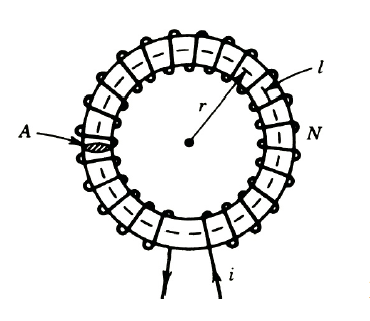
\includegraphics[width=5cm]{figures/toroid.PNG}
            \caption{Toroid}
            \label{fig:toroid}
        \end{figure}

    Consider a toroid (a ring shaped magnetic core), with wires wrapped around the entire circumference as shown in Fig \ref{fig:toroid}.
    When Current flow through the coil, the flux is mostly confined in the core material. The flux outside is called 
    leakage flux and it can usually be neglected. Consider a path at a radius r. The magnetic intensity on this path is H.
   
    
        \begin{align*}
            \oint H\cdot dl = Ni\\
            Hl = Ni\\
            H \cdot 2 \pi r = Ni
        \end{align*}
        where $N\cdot i$ is the magnetomotive force $mmf$.

        \begin{align*}
            Hl = Ni\\
            H = \frac{N}{l}\cdot i\\
            B = \frac{\mu Ni}{l} [Tesla]
        \end{align*}
    
    Assume that all the fluxes are confined in the toroid (no magnetic leakage). The magnetic flux across in the 
    cross section of the toroid is,
        \begin{align*}
            \Phi = \int{BdA}\\
            \Phi = BA[Wb]
        \end{align*}
    where B is the flux density in the core and A is the cross section area of the toroid.
    Let H be the magnetic intensity for this path,
        \begin{align*}
            \Phi &= \frac{\mu Ni}{l} A = \frac{Ni}{l/(\mu A)}\\
            &= \frac{Ni}{R}
        \end{align*}
    where $R$ is the reluctance of the magnetic path, and $\frac{1}{R}$ is called the permeance of the magnetic path.

    \subsection*{Magnetizing Curve}
        \begin{figure}[H]
            \centering
            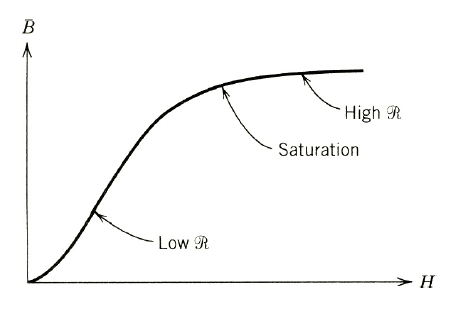
\includegraphics[width=5cm]{figures/magnetizing_curve.PNG}
            \caption{Magnetizing Curve}
            \label{fig:magnetizing_curve}
        \end{figure}


    If the magnetic intensity increased by increasing the current, the flux density in the core changes as shown in Figure \ref{fig:magnetizing_curve}.
    Before saturation, B increases at a rate of $\mu = \mu_{r}\mu_{o}$. After saturation, B increases at a rate of $\mu_{o}$.

    \subsection*{Example}
    \begin{figure}[H]
            \centering
            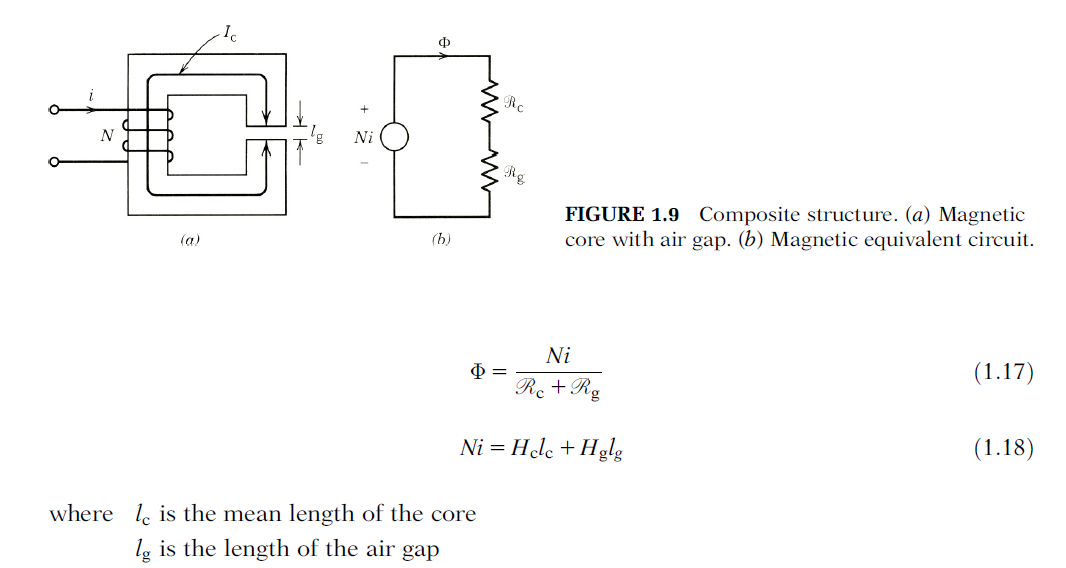
\includegraphics[width=12cm]{figures/magnetic_circuit_example1.PNG}
    \end{figure}

    \subsection*{Faraday's Law}
    A change in flux induces a voltage in the coil and the current flowing through the wire induces a 
    flux that opposes the original flux.
    \begin{equation*}
        e = -N\frac{d\Phi_{original}}{dt}
    \end{equation*}

    \subsection*{Self Inductance}
    \begin{align*}
        &L = \frac{N\Phi}{i}\\
        &Li = N\Phi \rightarrow \text{ flux linkage}
    \end{align*}

    \begin{align*}
        e = \frac{d(N\Phi)}{dt} &= \frac{dLi}{dt}\\
        & = \frac{Ldi}{dt} + \frac{idL}{dt} = \frac{Ldi}{dt}
    \end{align*}

    \begin{equation*}
        L = \frac{N \Phi }{i} = \frac{N^2}{Reluctance}
    \end{equation*}

    \subsection*{Lorentz Force}
    Moving a conductor in a magnetic field induces a current in that conductor.
    If the conductor is perpendicular to the magnetic field,
    \begin{equation*}
        F = i \cdot l \cdot B
    \end{equation*}


    \section*{DC Machine}
    \subsection*{Brushed Motor}

    \begin{figure}[H]
            \centering
            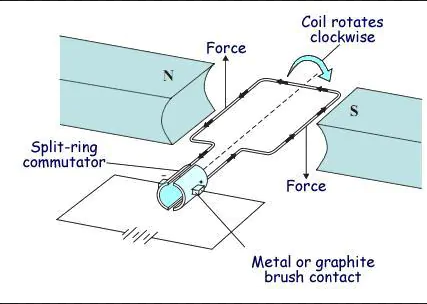
\includegraphics[width=5cm]{figures/brushed_motor.png}
    \end{figure}
    For dc motor, the flux $\Phi_{f}$ is established by the stator, this can be done with either a 
    permanent magnet or a field winding. In the field winding's case, the flux is proportional to 
    the current in the coils, where.
    \begin{equation*}
        \Phi_{f} = k_{f} I_{f}
    \end{equation*}

    The Electromagnetic torque of the motor is given by,
    \begin{align*}
        &T_{em} = F \cdot \frac{d}{2} \cdot 2\\
        &T_{em} = i\cdot l \cdot B \cdot d \cdot cos \theta \\
        &T_{em} = i \cdot A \cdot B \cdot cod \theta = i \Phi cos\theta\\
        &\boxed{T_{em} = k_{t} \Phi i_{a} } \text{ where $k_{t}$ is the motor torque constant}
    \end{align*}

    \subsubsection*{Back EMF}
    Since the armature(a conductor) is moving in the magnetic field, a voltage is induced 
    across the ends of the armature.
    At a speed of $\omega_{m}$, the induced $emf(electromotive force)\,e_{a}$ is,
    \begin{equation*}
        \boxed{e_{a} = lvB = A B \omega_{m} = k_{e}\Phi_{f} \omega_{m}} \\
    \end{equation*}
    where $k_{e}$ is the voltage constant of the motor.

    \subsection*{Power}
    Ideally, the power from the electrical domain is $\%$ transferred to the mechanical domain where,
    \begin{align*}
        &P_{e} = P_{m}\\
        &P_{e} = e_{a}i_{a} = k_{e} \Phi_{f} \omega_{m} i_{a}\\
        &P_{m} = \omega_{m}T_{em} =  k_{t} \Phi_{f} \omega_{m} i_{a}
    \end{align*}

    \subsection*{Electro-Mechanical Model}
    \begin{figure}[H]
            \centering
            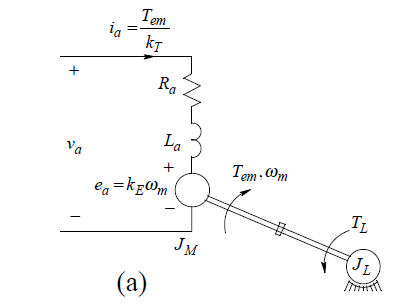
\includegraphics[width=5cm]{figures/elec-mech-model.png}
    \end{figure}
    In practice, a controllable voltage $v_{t}$ is applied to established $i_{a}$.
    \begin{equation*}
        V_{t} = e_{a} + i_{a}R_{a} + L_{a}\frac{di_{a}}{dt}
    \end{equation*}
    where $e_{a}$ is back emf, $R_{a}$ is armature resistance, and $L_{a}$ is armature inductance.

    Torque is given by,
    \begin{equation*}
        T_{em} = J_{L}\frac{d\omega_{m}}{dt} + B_{L}\omega_{m} + T_{L}(t)
    \end{equation*}
    where $J_{L}$ and $B_{L}$ are the total equivalent of inertia and damping, and $T_{L}$ is the load.

    \subsection*{Regenerative Braking}
    While the motor is in steady state, $V_{t} > E_{a}$ and $i_{a}$ is positive. If $V_{t}$ is decreased while 
    the motor is still moving forward, when $V_{t} < E_{a}$, $i_{a}$ is negative, creating a torque that 
    opposes the forward spinning, which decreases the motor speed. Since the speed of the motor is 
    decreasing, $e_{a}$ also decreases until the motor is completely stopped. When $i_{a}$ is negative, the motor is 
    a generator because the inertial energy of the motor is converted to current.

    \begin{figure}[H]
            \centering
            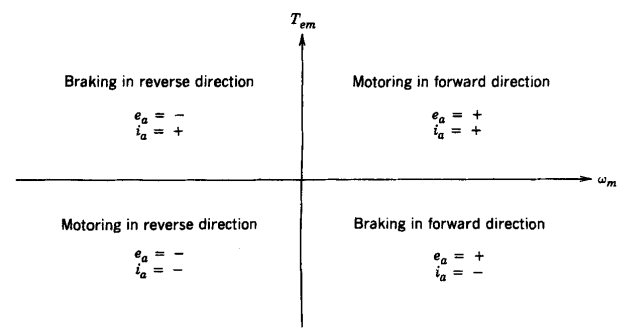
\includegraphics[width=10cm]{figures/4q_operation.png}
    \end{figure}

    \subsection*{Generating Magnetic Field}    
    \subsubsection*{Permanent Magnet}
    \begin{align*}
        &\Phi = \text{constant}\\
        &e_{a} = k_{e} \Phi_{f} \omega_{m} = k_{E} \omega_{m}\\
        &T_{em} = k_{t} \Phi_{f} i_{a} = k_{T} i_{a}
    \end{align*}

    In steady state, $\frac{di_{a}}{t} = 0$, 
    \begin{align*}
        &V_{t} = e_{a} + i_{a}R_{a} = k_{E} \omega_{m} + \frac{T_{em}}{k_{T}} R_{a}\\
        &\omega_{m} = \frac{1}{k_{E}} (V_{t} - \frac{R_{a}}{k_{T}}T_{em})
    \end{align*}

    \begin{figure}[H]
            \centering
            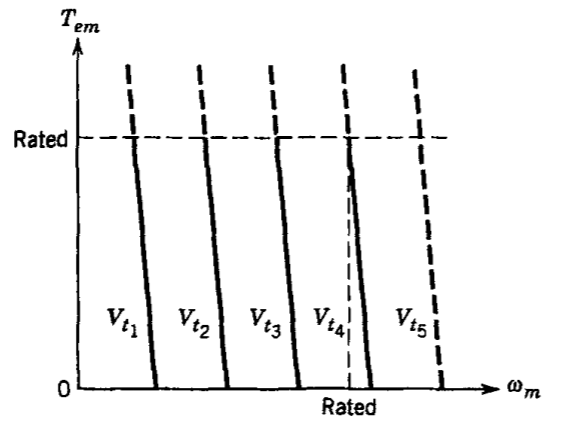
\includegraphics[width=8cm]{figures/t_omega_characteristic_dc.png}
    \end{figure}

        
    The armature current cannot exceeds the rated current, and therefore torque cannot exceeds the 
    rated value. On the other hand, speed cannot exceeds the rated value because it requires an input voltage that 
    exceeds the rated value. The rated values can be exceeded on a short-term bases but not long term.

    \subsubsection*{Field Winding}
        \begin{align*}
            &\Phi_{f} = k_{f}i_{f}\\
            &e_{a} = k_{e} k_{f} i_{f} \omega_{m}\\
            &T_{em} = k_{t} k_{f} i_{f} i_{a}
        \end{align*}

        \begin{align*}
            &V_{t} = e_{a} + i_{a}R_{a} = k_{E} \omega_{m} + \frac{T_{em}}{k_{T}} R_{a}\\
            &\omega_{m} = \frac{1}{\Phi_{f} k_{e}} (V_{t} - \frac{R_{a}}{\Phi_{f}k_{t}}T_{em})
        \end{align*}

    \section*{Induction Motor}        
    Induction motor is consisted of a stator and a rotor. The stator has three coils and when a three phase balanced 
    power is supplied to the coils, a rotating magnetic field is induced. A rotor is a current carrying loop of conductor placed within 
    the rotating magnetic field. The rotating magnetic field cuts through the rotor creating an emf on the loop causing the 
    loop to rotate. \par

    If the rotor rotates at the same speed as the magnetic field, the field no longer cuts through the conductors, and the rotor will decrease in 
    speed until the magnetic field is cutting through the conductors again. The rotor will never be able to catch up to the 
    rotating field.

    \subsection*{Number of Poles}
        \begin{equation*}
            rpm = \frac{120f_{in}}{p}
        \end{equation*}

    \subsection*{Synchronous Speed}
    The speed the magnetic field rotates at is called the synchronous speed.
        \begin{equation*}
            \omega_{s} = \frac{2\pi  / (p/2)}{1/f} = \frac{2}{p} \omega_{in}
        \end{equation*}
        where $\omega_{s}$ is the synchronous speed, p is the number of poles, and $\omega_{in}$ is the source frequency.

        \begin{equation*}
            rpm = 60 * \frac{\omega_{s}}{2\pi } = \frac{120}{f_{in}}
        \end{equation*}

    \subsection*{Air Gap Voltage}
    The rotating magnetic field causes an emf on the stator windings, $E_{ag}$, an air gap voltage is developed 
    in each of the windings. Assuming no leakage and no resistance in the stator windings.
    \begin{equation*}
        e_{ag} = N_{s} \frac{d \Phi_{ag}(t)}{dt} = N_{s} \omega \hat{\Phi}_{ag} cos( \omega t)
    \end{equation*}
    where $N_{s}$ is the number of turns per phase of the stator winding and $\Phi_{ag}(t)$ is the rotating flux and 
    $\hat{\Phi}_{ag}$ is the peak flux.

    \begin{align*}
        \Phi_{ag}(t) = \hat{\Phi}_{ag} sin(\omega t)\\
        \frac{d\Phi_{ag}}{dt} = \hat{\Phi}_{ag}(t) cos(\omega t)
    \end{align*}

    The rms air gap voltage is then,
    \begin{equation*}
        E_{ag} = k f \Phi_{ag}
    \end{equation*}
    where k is a constant.

    \subsection*{Slip Speed}
    \begin{equation*}
        \omega_{slip} = \omega_{synchronous} - \omega_{rotor}
    \end{equation*}
    
    \begin{equation*}
        \text{Slip} = \text{s} = \frac{\omega_{slip}}{\omega_{synchronous}}
    \end{equation*}

    \subsection*{Rotor Voltage}
    The induced voltage on the rotor is proportional to the slip speed.
    \begin{equation*}
        E_{r} = k f_{slip} \Phi_{ag}
    \end{equation*}
    which is similar to $E_{ag}$ but the speed is the slip speed which is the relative speed between the 
    rotor and the rotating flux. k is the same constant as the k that appeared in $E_{ag}$.

    \begin{equation*}
        E_{ag} = sE_{r}
    \end{equation*}
    
    The rotor voltage induces a current at the slip frequency in the the rotor, and therefore
    \begin{equation*}
        E_{r} = R_{rotor}i_{rotor} + j 2 \pi f_{slip} L_{leakage_rotor} i_{rotor}
    \end{equation*}

    \subsection*{Per Phase Rotor-Stator Circuit}
        \begin{figure}[H]
            \centering
            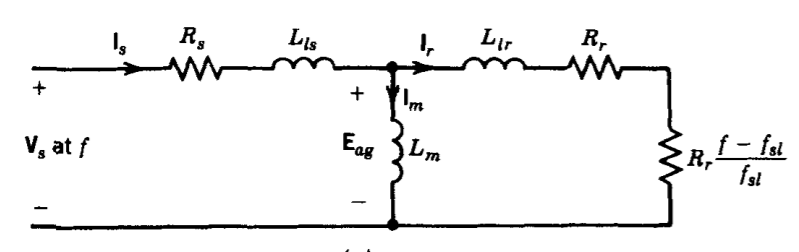
\includegraphics[width=8cm]{figures/rotor_stator_circuit.png}
        \end{figure}

        The total current drawn by the stator is the sum of the magnetizing current and the rotor current.
        The magnetizing current produces the rotating flux and the rotor current produces electromagnetic torque.

        \begin{figure}[H]
                \centering
                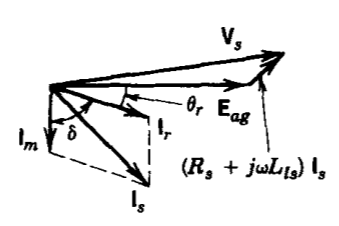
\includegraphics[width=8cm]{figures/rotor_stator_phasor.png}
        \end{figure}

        \begin{align*}        
            &\text{power factor } = \theta_{rotor} = tan^{-1}(\frac{2\pi f_{slip} L_{leakage_rotor}}{R_{rotor}})\\
            &\text{torque angle } = \delta = 90\degree + \theta_{rotor}
        \end{align*}

        \begin{equation*}
            V_{source} = E_{ag} + (R_{s} + j2\pi f L_{leakage_stator}) I_{stator}
        \end{equation*}

        \begin{equation*}
            T_{em} = k_{4}\Phi_{ag}I_{rotor}sin(\delta)
        \end{equation*}

        Usually, $2\pi f_{slip}L_{leakage_rotor} \ll R_{rotor}$ and therefore, $\delta \sim 90\degree $
        \begin{align*}
            &T_{em} = k_{4}\Phi_{ag}I_{rotor}\\
            &I_{rotor} \sim k_{5}\Phi_{ag} f_{slip}\\
            &T_{em} = k_{6} \Phi^{2}_{ag} f_{slip}\\
        \end{align*}

    \subsection*{Power}
        \begin{align*}
            &P_{rotor} = 3 R_{rotor} I_{rotor}^{2}\\
            &P_{ag} = 3 \frac{f_{input}}{f_{slip}} R_{rotor} I_{rotor}^{2}\\
            &P_{em} = P_{ag} - P_{rotor} 
        \end{align*}

        \begin{equation*}
            T_{em} = \frac{P_{em}}{\omega_{rotor}} = \frac{P_{ag}}{\omega_{synchronous}}
        \end{equation*}


   



    





    

    


\end{document}